\section{Well-typedeness and normalisation of $\lambda$-terms in first-order logic}
\label{sec:eval}


\newcommand{\NonLinTerms}[2]{\Lambda_{#1} #2}
 \newcommand{\rlambda}{\ranked{\Lambda}}
 \newcommand{\rlambdalin}{\ranked{\Lambda^{\sf{lin}}}}
 \newcommand{\rlambdathin}{\ranked{\Lambda^{\sf{thin}}}}


\newcommand{\thinterm}[1]{\ranked{\mathsf{Thin}_{#1}}}

\subsection{Well-typedeness}
A natural question to ask about $\lambda$-terms in our framework is whether their well-typedeness is a first-order property. Without restriction on terms, the answer is negative as shown by 
Example~\ref{ex:exponential}.
%the following example.
%
%\begin{example}
%Consider the set of typed variables $X=\{x:o, y:o\rightarrow o, z:o\rightarrow(o\rightarrow o), t:o, u:o\rightarrow o\}$ and the set of $\lambda$-terms $(M_n)_{n\in \mathbb{N}}$ defined by induction as follows: 
%\begin{align*}
%M_0 &= u(yx)\\
%M_{n+1}&= (\lambda y.\lambda x. M_n)(z(yx))
%\end{align*}
%The type of $M_n$ is $o^n\rightarrow o$ where $o^n\rightarrow o$ stands for $\underbrace{o\rightarrow\dots\rightarrow o}_{n \text{ times}}\rightarrow o$ when $n>0$ and for $o$ otherwise. 
%
%Consider now the set of $\lambda$-terms $(L_{m,n})_{m,n\in \mathbb{N}}$ defined by induction on $m$ as follows:
%\begin{align*}
%L_{0,n}&= M_n \\
%L_{m+1, n}&=L_{m,n}t
%\end{align*}
%When $m\leq n$, the $\lambda$-term $L_{m,n}$ is well-typed and its type is $o^{m-n}\rightarrow o$, otherwise it is not well-typed. If well-typedeness was an fo property, we would be able to make such tests on natural numbers which is clearely not the case. 
%\end{example}
%
When we restrict our attention to those $\lambda$-terms whose subterms have types in a fixed finite set $S$, well-typedeness becomes a first-order property. Note that contrarily to $\beta$-reduction, well-typedeness does not require linearity to be in fo.

\begin{proposition}\label{prop:WellTypedFo}
    For every typed set $X$ and every finite set $S$ of simple types, the tree language 
    \begin{align*}
    \NonLinTerms S X  := \set{ M \in \trees \lamrank X : \text{$M$ is well-typed and all subterms have type in $S$}}
    \end{align*}
    is first-order definable 
\end{proposition}

To prove this property, we will start by showing that for $\lambda$-terms in $\NonLinTerms S X$ (that is if we already know that a $\lambda$-term is well-typed and that all its sub-terms have types in $S$) checking if their type is $\tau$, where $\tau$ is a type in $S$, is a first order property:
\begin{lemma}\label{lem:IsTypeTauFo}
For every simple type $\tau$ in $S$, there is a first-order query $\varphi_\tau$ such that:
$$ \forall M\in \NonLinTerms S X \qquad M,u \models \varphi_\tau \Longleftrightarrow M|_u:\tau$$
where $M|_u$ is the subtree of $M$ rooted in $u$. 
\end{lemma}
Before establishing this lemma, let us see how Proposition~\ref{prop:WellTypedFo} can be derived from it. Suppose for convenience that $S$ is downward closed. For every type $\tau$ in $S$, let $\varphi_\tau$ be the formula given by Lemma~\ref{lem:IsTypeTauFo}. In the following, we use the binary formula
 $\mathsf{Succ}_{i}(u,v)$ which is valid when $v$ is the $i$-th child of $u$, and which is easily expressible in first-order logic.
 \smallskip
 
Consider the unary formula $\mathsf{Lambda}(u)$, which expresses that $u$ is a binder node, that its type and the type of its child match well and both belong to $S$: 
\begin{align*}
\mathsf{Lambda}(u) := \bigvee_{\substack{\sigma\rightarrow\tau \in S\\x:\sigma}} \underbrace{\lambda x(u)}_{\substack{\text{$u$ has label $\lambda x$}}} \wedge \underbrace{\varphi_{\sigma\rightarrow\tau}(u)}_{\substack{\text{$u$ has type $\sigma\rightarrow\tau$}}}  \wedge \underbrace{\exists v\ \ \mathrm{Succ}_1(u, v) \wedge \varphi_\tau (v)}_{\substack{\text{the child of $u$ has type $\tau$}}}
\end{align*}

Similarly, consider the unary formula $\mathsf{Application}(u)$ which checks that a node is an application node, that the type of its children match well and that both belong to $S$: 
\begin{align*}
\mathsf{Application}(u) := \bigvee_{\sigma\rightarrow\tau \in S} \underbrace{@(u)}_{\substack{\text{$u$ has label @}}}  \wedge \exists v, w\ \ \underbrace{\mathrm{Succ}_1(u, v) \wedge \varphi_{\sigma\rightarrow\tau} (v)}_{\substack{\text{the left child of $u$ has type $\sigma\rightarrow\tau$}}} \wedge \underbrace{\mathrm{Succ}_2(u, w) \wedge \varphi_{\sigma} (w)}_{\substack{\text{the right child of $u$ has type $\sigma$}}}
\end{align*}

Finally, consider the formula $\mathsf{Variable}(u)$, which expresses that $u$ is a variable node, whose type is in $S$:
\begin{align*}
\mathsf{Variable}(u) :=  \bigvee_{x:\sigma\in S}\underbrace{x(u)}_{\substack{\text{$u$ has label $x$}}} 
\end{align*}  
We claim that the following (nullary) formula $\phi$ recognizes the tree language $\NonLinTerms S X$
\begin{align*}
\phi = \forall u.\ \mathsf{Variable}(u)\ \vee\ \mathsf{Lambda}(u)\ \vee\  \mathsf{Application}(u)
\end{align*}
If a $\lambda$-term is in $\NonLinTerms S X$, then it clearly satisfies $\phi$. Suppose by contradiction that there is a $\lambda$-term $M$ which is not in $\NonLinTerms S X$ and yet satisfies $\phi$. Let $u$  be the deapest node of $M$ which is not in $\NonLinTerms S X$ (we identify in this proof a node $u$ and the subterm $M|_u$). In particular, the descendents of $u$ are all in $\NonLinTerms S X$. The node $u$ cannot be a variable, since variable nodes are well-typed and their type is in $S$ by the first disjunct of $\phi$.  If $u$ was labeled by $\lambda x$, where $x$ is of type $\sigma$, then by the second disjunct of $\phi$ there is a type $\tau$ such that $\sigma\rightarrow\tau\in S$ and the child $v$ of $u$  satisfies $\varphi_\tau$. Since $v$ is in $\NonLinTerms S X$, its type is $\tau$ by Lemma~\ref{lem:IsTypeTauFo}. Hence $u$ is well-typed and its type is $\sigma\rightarrow\tau\in S$. As a consequence $u$ is in $\NonLinTerms S X$ which is a contradiction.  Finally, if $u$ was labeled by $@$, then by the third disjunct of $\phi$, its two children $u_1$ and $u_2$
would satisfy respectively $\varphi_{\sigma\rightarrow\tau}$ and  $\varphi_{\sigma}$ and by Lemma~\ref{lem:IsTypeTauFo} they are of type $\sigma\rightarrow\tau$ and $\sigma$ respectively. The node $u$ is then well-typed and its type is $\tau$ (which is a type of $S$ thanks to downward closeness). As a consequence, $u$ is in $\NonLinTerms S X$, wich gives a contradiction and concludes the proof.
 \smallskip
 
We can go back now to the proof of Lemma~\ref{lem:IsTypeTauFo}.
\begin{proof}[Proof of Lemma~\ref{lem:IsTypeTauFo}]
Let us show that the following unary query is expressible in first-order logic
\begin{center}
''if $t$ is a $\lambda$-term of $\NonLinTerms s X$, then its type is $\tau$ ``:
\end{center}
 For that, notice that the type of a well-typed term depends only on its left-most branch. In fact, the type of a term is exactly the type of its left-most branch in the following sens.

Consider the (unranked) alphabet $ X_\lambda:= X\cup \{@, \lambda x | x\in X\}$. We can equip the words over $X_\lambda$ with the following typing rules:
$$\frac{}{x: \sigma} \qquad \frac{u:\tau}{u\lambda x: \sigma\rightarrow \tau} \qquad \frac{u:\sigma\rightarrow\tau}{u@:\tau}\qquad\text{(where $x$ is of type $\sigma$ and $\sigma,\tau \in S$)}$$
We say that $w$ is of type $\tau$ and write $w:\tau$ if there is a typing derivation for $w:\tau$.

We can associate to every branch of a $\lambda$-term a word over $X_\lambda$ corresponding to the sequence of its labels read bottom-up. By induction on $\lambda$-terms, we can easily show that the type of a $\lambda$-term is the type of the word corresponding to its leftmost branch. 

By this last observation, we can reduce the query asking if the type of a term is $\tau$, to the same query but on $X_\lambda$ words. To show that the former is a first-order query, it is then sufficient to show that the following word language 
\begin{align*}
W_\tau = \{w\in X.\{@, \lambda x | x\in X\}^*\ |\ w:\tau \} 
\end{align*}
is first-order definable, or equivalently that  $W_\tau$ is recognized by a counter-free non-deterministic finite automaton. For that we proceed as follows: first, we show that $W_\tau$ is recognized by a pushdown automaton $P_\tau$. Then we will show that the stack height of $P_\tau$ is bounded, thus it can be turned into a deterministic finite automaton $D_\tau$. Finally, we show that the obtained automaton $D_\tau$ is actually counter-free.  

%For a formal definition of pushdown automata (PDA) and (counter-free) non-deterministic finite automata (NFA) see~\ref{}.

Consider the pushdown automaton $P_\tau$ whose
\begin{itemize}
\item  set of states is $\{i, p, f\}$, where $i$ is the initial state and $f$ the accepting state;
\item input alphabet is the alphabet $X_\lambda$;
\item stack alphabet is the set of types $S$;
\item and whose transition function is described as follows:
\begin{itemize}
\item If the automaton is in the initial state $i$ with an empty stack, and if the symbol it reads is a variable $x$ of type $\sigma_1\rightarrow\dots\rightarrow\sigma_n$, then we go to the state $p$ and push the symbols $\sigma_n,\dots,\sigma_1$  in the stack in this order. The toplevel symbol of the stack is then $\sigma_1$.
\item If the automaton is in the state $p$ and it reads the symbol $\lambda y$, where $y$ is of type $\sigma$, then push the symbol $\sigma$ in the stack, and stay in the state $p$.
\item  If the automaton is in the state $p$,  if it reads the symbol $@$ and if the stack is non empty, then pop the top-level symbol and stay in the state $p$.
\item If the automaton reachs the end of the word being in state $p$, and if the stack contains only the symbol $\tau$, then pop it and go to the final state $f$.  
\end{itemize}
\end{itemize}
A word $w$ is accepted by $P_\tau$ if there is a run that reaches the end of $w$ in the accepting state $f$ with an empty stack. We write $(r, s)\xrightarrow{w} (r', s')$ if there is a run over the word $w$ which starts in the state $r\in\set{i, p,f}$ and with a stack $s$ and ends up in the state $r'\in\set{i, p,f}$ and with a stack $s'$.


By induction on the lenght of the word $w$, we can easily show that:
\begin{lemma}
For every word $w\in X.\{@,\lambda x | x\in X \}^*$, we have that:
 $$(i, \epsilon)\xrightarrow{w} (p, \sigma_n\dots\sigma_1) \qquad\text{iff} \qquad 
w:\sigma_1\rightarrow\dots\rightarrow\sigma_n$$ 
\end{lemma}

A direct consequence of this lemma is that $P_\tau$ recognizes $W_\tau$. Another direct consequence is that the stack height of $P_\tau$ is bounded by $m$, the size of the longuest type in $S$. Thus $P_\tau$ can be turned into a DFA $D_\tau$, by encoding the stack information in the states. More precisely, the states of $D_\tau$ are pairs $(r,s)$ where $r\in \set{i,p,f}$ and $s$ is a stack of height at most $m$, the initial state is $(i,\epsilon)$ and there is a transition $(r,s)\xrightarrow{a}(r',s')$ where $a\in X_\lambda\cup\{\epsilon\}$ if there is a corresponding run in $P_\tau$. We show in the following that $D_\tau$ is counter-free. 

Let us start with some observations. In the pushdown automaton $P_\tau$, the effect of a word $w$ on a stack $s$, starting from the state $p$ is the following: it erases the first $n$ top level elements of $s$, and replaces them by a word $u$. The number $n$ and the word $u$ do not depend on the stack $s$ but only on the word $w$. This is exactly what the following lemma claims.

\begin{lemma}
For every word $w$ over ${X_\lambda}^*$, there is a natural number $n$ and a word $u\in S^*$ such that if $(p,s)\xrightarrow{w}(p,s')$ then $s$ and $s'$ can be decomposed as follows:
$$s=t.v,\qquad s'=t.u\qquad \text{ and }\qquad |v|=n.$$
\end{lemma}
The proof is an easy induction on the lenght of $w$. As a consequence we have that:
\begin{itemize}
\item If $(p,s_1)\xrightarrow{w}(p,s_2)\xrightarrow{w}(p,s_3)$ and $|s_2|>|s_1|$ then $|s_3|>|s_2|$.
\item If $(p,s_1)\xrightarrow{w}(p,s_2)\xrightarrow{w}(p,s_3)$ and $|s_2|<|s_1|$ then $|s_3|<|s_2|$.
\item If $(p,s_1)\xrightarrow{w}(p,s_2)\xrightarrow{w}(p,s_3)$ and $|s_2|=|s_1|$ then $s_3 =s_2$.
\end{itemize}

Let us show that $D_\tau$ is counter-free. Suppose by contradiction that there is a word $w$ and pairwise distinct stacks $s_1,\dots, s_n$ such that 
\begin{align*}
(p,s_1)\xrightarrow{w}(p,s_2)\xrightarrow{w}\dots(p,s_n)\xrightarrow{w}(p,s_1).
\end{align*} 
By the first two properties above, we have necessarily that 
\begin{align*}
|s_1|=\dots=|s_n|
\end{align*}
 Thus by the third property, we have that 
\begin{align*}
 s_1=\dots=s_n
\end{align*} 
 which concludes the proof.
\end{proof}



\subsection{Evaluation of linear $\lambda$-terms}

In this section we show that computing the normal form of $\linterm S X$ terms (that is well-typed linear $\lambda$-terms whose subterms have all types in $S$) is a derivable function:

 \begin{proposition}\label{prop:one-register} 
    For every typed set $X$ and every finite set $S$ of simple types, the function 
    \begin{align*}
        M \in  \linterm S X \qquad \mapsto \qquad \text{normal form of $M$} \in  \linterm S X
    \end{align*}
    is derivable.
\end{proposition}

The proof proceeds by induction on the set of types $S$. The main observation is that, if the evaluation of a redex of type $\sigma\rightarrow \tau$ creates new redexes, then their types are either $\sigma$ or $\tau$, they are in particular in $S\setminus\{\sigma\rightarrow\tau\}$. Thus, we only need to show that the function that evaluates all the redexes of a fixed type is derivable. As we only create stricty smaller redexes, we need to iterate this process only finitely many times, the bound being the size of $S$. 

  Since we have only finitely many typed variables, it is enough to show that the function that evaluates all the redexes of a fixed type $\sigma$ and a fixed variable $x$ is derivable. This will be our goal in the rest of this section.

\begin{theorem}\label{thm:evalOneType}
 For every typed set $X$, every finite set $S$ of simple types and every $x\in X$ and $\sigma\in S$, the function 
    \begin{align*}
        M \in  \linterm S X \quad \mapsto \quad N \in \linterm S X \text{ obtained by reducing all the $x$-redexes of type $\sigma$ in $M$} 
    \end{align*}
    is derivable.
\end{theorem}



\subsubsection{Evaluation of thin $\lambda$-terms}

We start by showing that the evaluation of a restricted class of linear $\lambda$-terms, which we call thin, is derivable.   

\begin{definition}[Thin $\lambda$-terms]
We say that the node of a $\lambda$-term is \emph{branching} if its has at least two children which are not ports.
 
A \emph{thin $\lambda$-term} is a term from $\linterm S X$ in which, if a node is branching, then it is an application node of a redex. We denote by $\thinterm S X$ the set of thin $\lambda$-terms.
\end{definition}

Since thin $\lambda$-terms branch only on redexes, the result of their evaluation is a ''word`` (in the sens that every node has at most one non-port child).  We will show that this word can actually be obtained by a pre-order traversal of the original $\lambda$-term. We will then use the basic pre-order traversal  function to show that evaluation of thin $\lambda$-terms is derivable. 

The left $\lambda$-term belwo is thin. The coloured nodes are the ones which are not redexes, nor the variables they bind. The right $\lambda$-term is its normal form,  where we can see that the order of the nodes is the pre-order traversal of the original $\lambda$-term.  
\begin{center}
		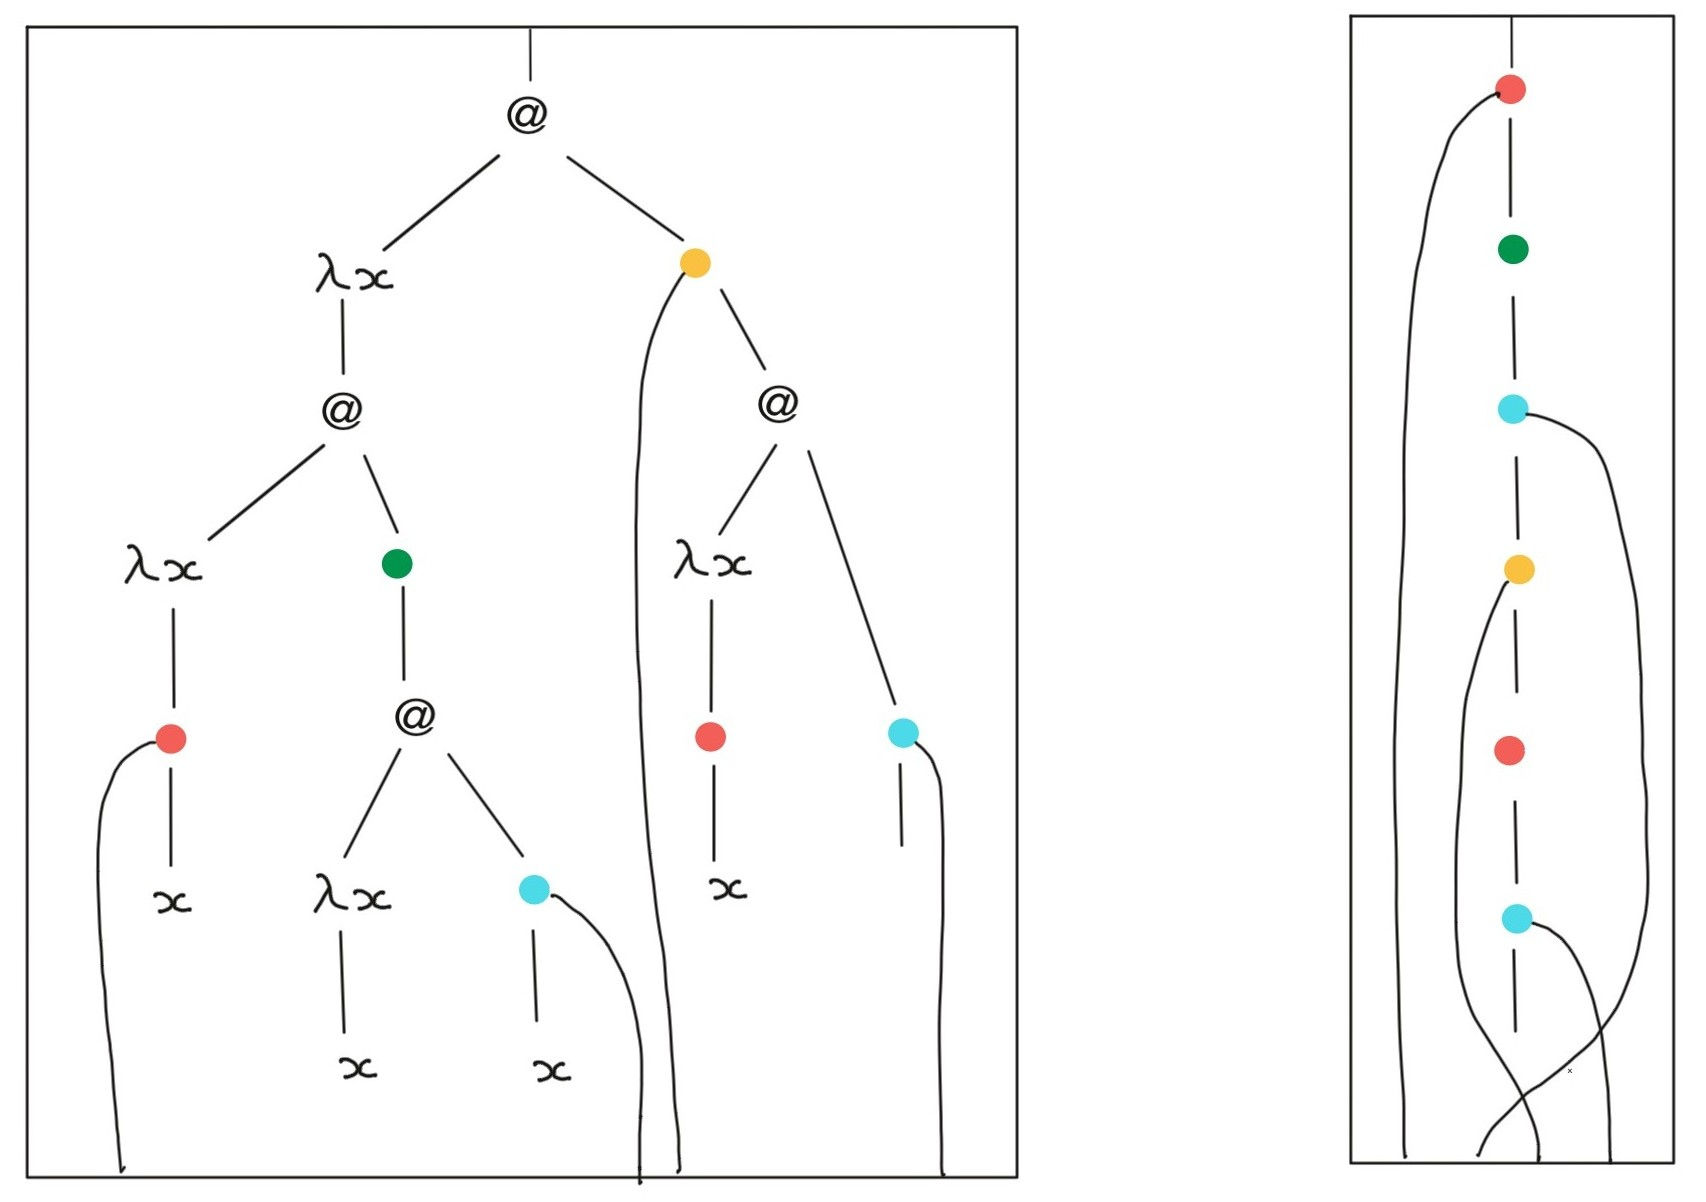
\includegraphics[scale=.15]{MyPic10.jpg}
		\end{center}

\begin{proposition}\label{prop:EvaluateThin}
 For every typed set $X$ and every finite set $S$ of simple types, the function 
    \begin{align*}
        M \in  \thinterm S X \qquad \mapsto \qquad \text{normal form of $M$} \in  \thinterm S X
    \end{align*}
    is derivable.
\end{proposition}

\begin{proof}
Let us show that the evaluation of thin $\lambda$-terms is derivable. We will consider an additional hypothesis on thin $\lambda$-terms:
\begin{center}
\textit{If a node is an application node of a redex, then it is branching.}$\qquad\qquad (H)$
\end{center}
Hypothesis $(H)$ is the converse of the condition on thin $\lambda$-terms. We will first show that normalisation of thin $\lambda$-terms with this additional condition (let us call them strongly thin $\lambda$-terms) is derivable, then we will show later how to get rid of it.

Let $t$ be a strongly thin $\lambda$-term and let $u$ be its normal form. As noticed before, $u$ has the shape of a word. Moreover, since $t$ is linear, the nodes of $u$ are exactly the nodes of $t$ which are not redexes, nor the variable nodes bound by these redexes. We show that:
\noindent \begin{enumerate}
\item The order in which the inner nodes (ie. non ports) of $u$ appear is the tree order of $t$.
\item Let $n$ be a node of $u$ and $m$ be its corresponding node in $t$. The port $p$ of $u$ is the $i^{th}$ child of $n$ if and only if the port $p$ of $t$ is the $i^{th}$ child of $m$.  
\end{enumerate} 

To establish the second claim, it is enough to show it for one step of $\beta$-reduction. But this last point is clear by a simple analysis of $\beta$-reduction, as far as we consider that the right child of the $@$ node of every redex is not a port. This is is guaranteed by the condition $(H)$ of strongly thin $\lambda$-terms. 


To establish the first claim, we need the following lemma.
\begin{lemma}\label{lem:internalLemma}
Let $t$ be a thin $\lambda$-term, let $m$ be the binder node of a redex of $t$ and let $n$ be the node of the variable bound by $m$.

The node $n$ is the greatest node in the subterm $t|_m$ wrt. the tree order. 
\end{lemma}
\begin{proof}
We proceed by induction on the lenght of the path between $m$ and $n$. When it is $0$ the result is clear. Suppose now that it is strictly greater than $0$ and that there is a node $o$ which is strictly greater than $n$. We take $o$ to be the smallest node which is greater than $n$. Since $t$ is thin, the least common ancestor $l$ between $n$ and $o$ is an application node of a redex. Since $n$ is smaller than $o$, $n$ is the left descendant  of $l$, in other words it is the descendant of the left child $p$
of $l$, which is a binder. The node $m, n, o$ and $p$ are illustrated below:
\begin{center}
		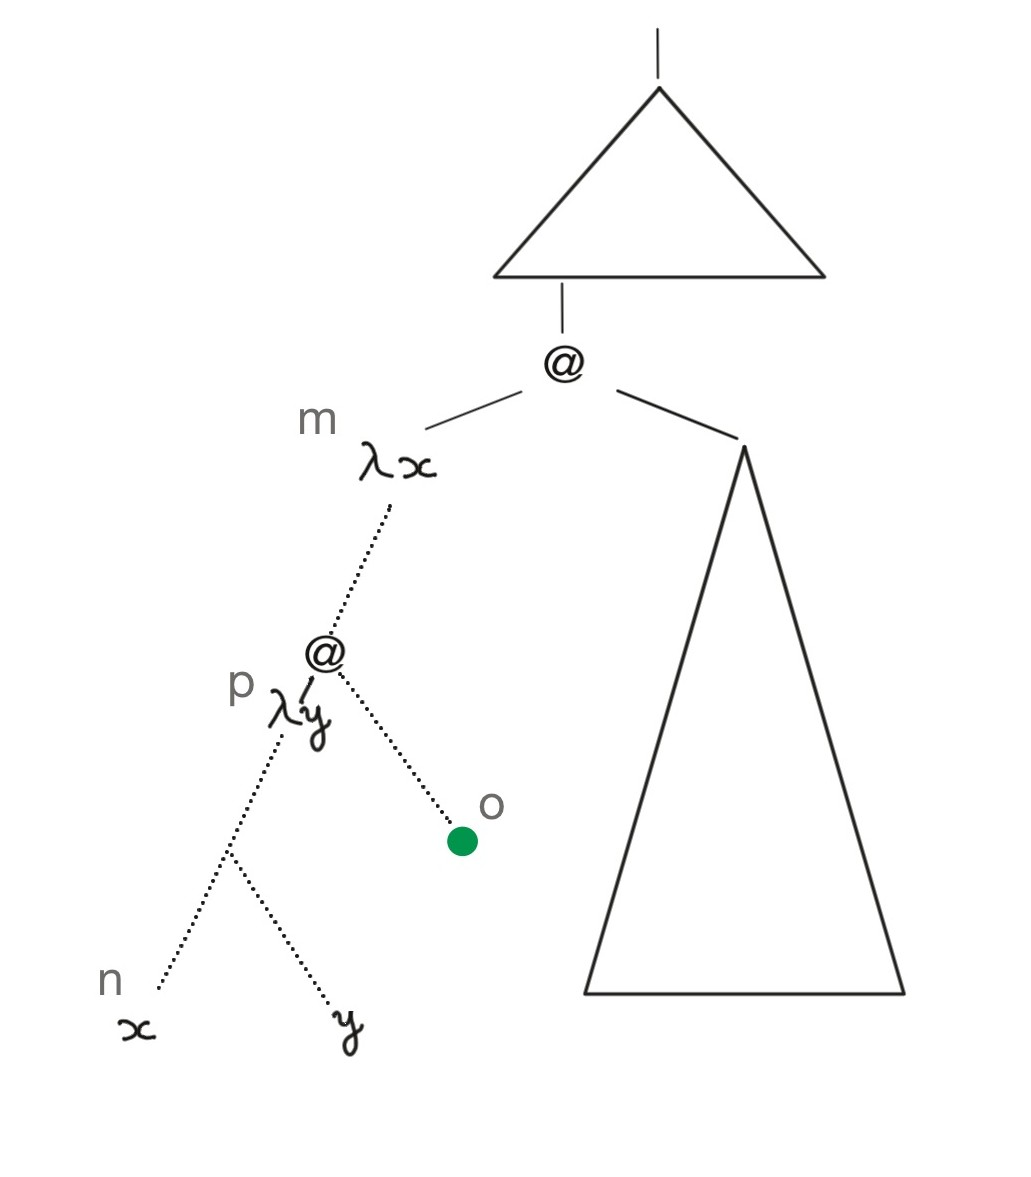
\includegraphics[scale=.15]{MyPic11.jpg}
\end{center} 
 By induction hypothesis, the variable
bound by $p$ is strictly greater than $n$. Is is also strictly smaller than $o$, which gives a contradiction and concludes the proof. 
\end{proof}

Let us go back to the proof of the first claim. Consider two inner nodes $n, m$ of $t$ which are also nodes of $u$, and such that $m$ is smaller than $n$ is the tree order of $t$. We show that $n$ is a descendant of $m$ in $u$. There is two cases to consider:

\textbf{Case 1.} Either $n$ is a descendent of $m$ in $t$, in this case we can conclude easily since $\beta$-reduction preserves the descendent relation. Indeed, by a small analysis of $\beta$-reduction, one can notice that a reduction step may extend the descendent relation, but can never change (or break) the order of two comparable nodes in the original $\lambda$-term.    

\textbf{Case 2.} Otherwise, let us consider the lowest common ancestor $p$ of $m$ and $n$. We proceed by induction on the lenght of the path between $m$ and $p$. By definition of thin $\lambda$-terms, since $p$ is branching it is necessarily an $@$ node, whose left child $q$ is a binder node, let us say $\lambda x$. 
By Lemma~\ref{lem:internalLemma}, $m$ is smaller wrt. the tree order than the node $r$ of the variable bound by $q$ . 
We are then left with the following two situations. The first case, illustrated by the left figure below, is when $r$ is a descendant of $m$ in $t$. In this case, after one reduction step $n$ will be a desendant of of $m$. The other case is when $m$ is in the left of $r$ in $t$, as illustrated by the right figure below. In this case, after one reduction step, the lowest common ancestor between $m$ and $n$ will be a descendant of $p$, and we can conclude by induction hypothesis. This concludes the proof of the first claim.

$\qquad\qquad\quad$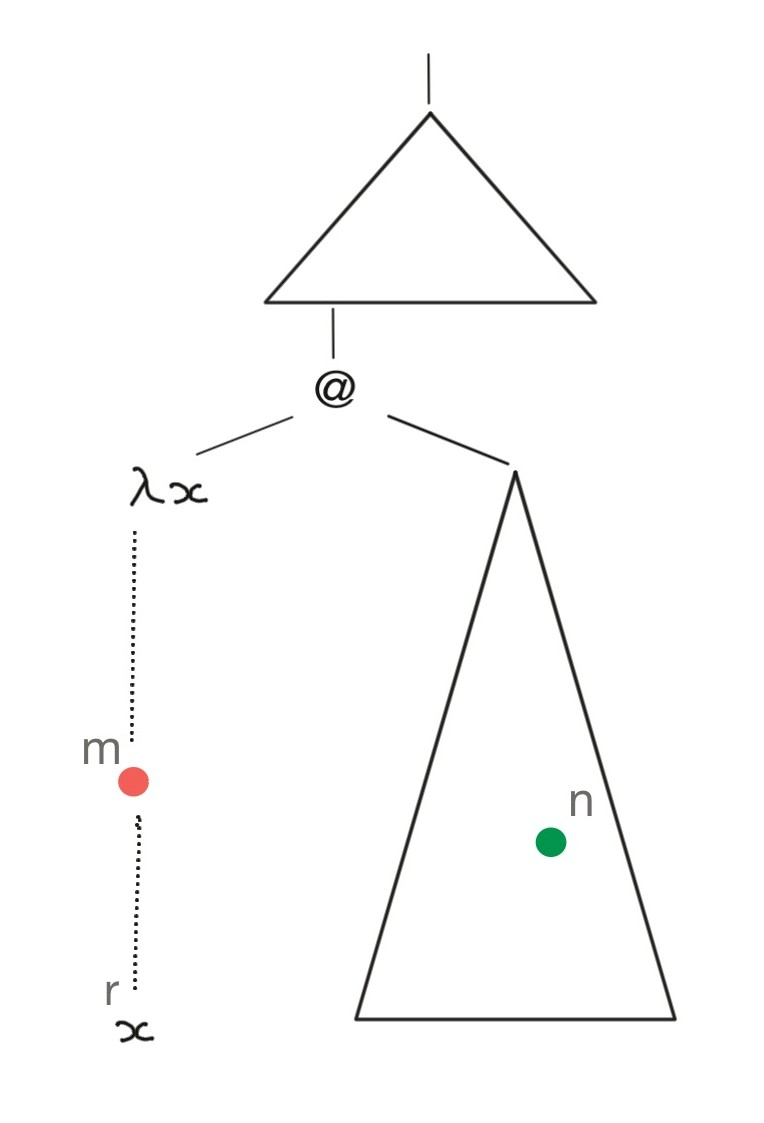
\includegraphics[scale=.15]{MyPic12.jpg}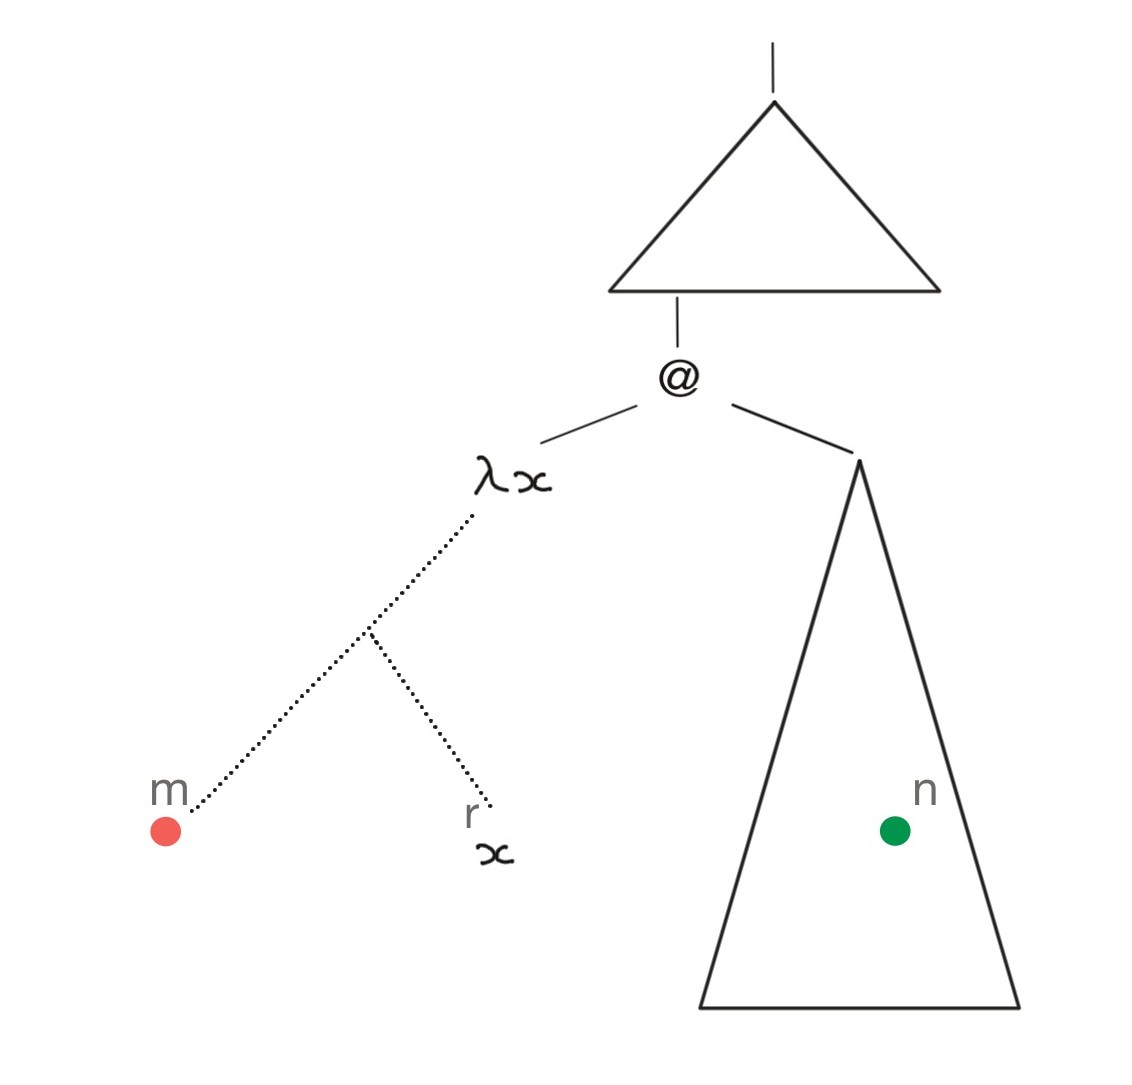
\includegraphics[scale=.15]{MyPic13.jpg}
%\end{center}    

Using these ingredients, let us construct a derivable function which computes the normal form of thin $\lambda$-terms. We illustrate this construction on a $\tmonad(X^\lambda)$ term $t$ below which will be our running example in this proof. 

%   
\begin{enumerate}
\item
We start by distinguishing the redexes of $t$ and their bound variables from the other nodes. For that, we apply the characteristic function of the following first-order query $\varphi$:
    \begin{center}
    ``The node $u$ is a redex or a variable bound by a redex''
    \end{center}
    This query is first-order expressible. Indeed being a redex is the disjunction of the following two queries
$$\begin{array}{rl}
@\mathsf{Redex}(u) = & @(u) \wedge \exists v \ \mathrm{Child}_1(u,v) \wedge \bigvee_{x\in X}\lambda x(v)\\
\lambda\mathsf{Redex}(u)=& \lambda x(u) \wedge \exists v \ \mathrm{Child}_1(v,u) \wedge @(v) 
\end{array}$$
where $@\mathsf{Redex}(u)$ says that $u$ is the application node of a redex, and $\lambda\mathsf{Redex}(u)$ says that it is the abstraction node of a redex. Being a variable bound by a redex can be expressed by the formula $X\mathsf{Redex}(u)$ defined as follows
%$$
%\begin{array}{ll}
\begin{align*}
X\mathsf{Redex}(u)&=\bigvee_{x\in X} x(u) \wedge \exists v\ \lambda\mathsf{Redex}(v) \wedge v\ \mathsf{binds}\ u\\
\end{align*}
%\end{array}
%$$    
Where the formula $u\ \mathsf{binds}\ v$, defined below,  is a binary first-order query expressing that the node $u$ is an abstraction node that binds $v$.
 \begin{align*}
 \bigvee_{x\in X} \lambda x(u) \wedge x(v) \wedge u<v\wedge \forall u<w<v\ \neg \lambda x(w)
 \end{align*}

The query $\varphi$ being first-order, its characteristic function is derivable thanks to Proposition~\ref{prop:forat}. 

When we apply this step to our example term $t$,  we get the $\ranked{\tmonad(X^\lambda+X^\lambda)}$ term below. We coloured in red the nodes belonging to the first copy of $\ranked{X^\lambda}$, that is the nodes satisfying the query $\varphi$. These nodes are the ones that will desappear in the normal form of $t$. 
\begin{center}
Picture
\end{center}
\item After that, we apply the pre-order traversal function 
\begin{align*}
            \ranked{\preorder : \tmonad (X^\lambda+X^\lambda) \to \tmonad (X^\lambda+X^\lambda + \set{\grayball, \grayballbin})}
\end{align*}
After this step, our initial term becomes
\begin{center}
Picture
\end{center}  
In this term, the nodes of the normal form appear in the right order thanks to the first claim. We only need to get rid of the redexes and the variable nodes that participated in the computation of the normal form (that is the ones coloured in red) together with the nodes $\grayball$ and $\grayballbin$ introduced by the pre-order traversal. 
\item For this purpose, we apply the function $\ranked{\mathsf{Tagg\text{-}Parent}_{\set{\grayballbin}}}$ from Example~\ref{ex:Tagg}
\begin{align*}
\ranked{\mathsf{Tagg\text{-}Parent}_{\set{\grayballbin}}: \tmonad (X^\lambda+X^\lambda + \set{\grayball, \grayballbin}) \to \tmonad (X^\lambda+X^\lambda + \set{\grayball, \grayballbin}+\#) }
\end{align*}
 which adds the unary symbol $\#$ as the parent of every node $\grayballbin$. Then we apply the factorisation $\ancfact$
 to separate the symbol $\#$ from the others:
 \begin{align*}
 \ranked{\ancfact : \tmonad (X^\lambda+X^\lambda + \set{\grayball, \grayballbin}+\#) \to \tmonad (\tmonad(X^\lambda+X^\lambda + \set{\grayball, \grayballbin})+\tmonad\set{\#}))}
 \end{align*}
 
 After this step, our example term becoms    
\begin{center}
Picture
\end{center}
\item Now consider the constant function
 \begin{align*}
 \ranked{f: \tmonad\set{\#} \to \tmonad(X^\lambda+X^\lambda+\set{\grayball, \grayballbin})}
 \end{align*}
 which assigns the empty term (that is the term $x_1$) to every term. And consider the function 
 \begin{align*}
 \ranked{g: \tmonad(X^\lambda+X^\lambda+\set{\grayball, \grayballbin}) \to \tmonad(X^\lambda+X^\lambda+\set{\grayball, \grayballbin}+\set{\#})}
 \end{align*}
 which is the identity function, except for the following finite set of terms for which it is defined as  
\begin{center}
Picture
\end{center}
\item We apply $f$ to the $\tmonad\set{\#}$ factors and $g$ to the other factors, then we flat the resulting term. We obtain the following $\tmonad(X^\lambda+X^\lambda+\set{\grayball, \grayballbin})$ term, which is  the normal form of $t$. 
\begin{center}

\end{center}
Note that we obtained the desired term, but not with the desired type. To obtain a term in $\ranked{\tmonad{X^\lambda}}$, we lift the co-pairing of the identity function (twice)
\begin{align*}
\mathsf{identity}: X^\lambda \to X^\lambda
\end{align*}
with the function $h_x$, where $x$ is a variable in $X$
\begin{align*}
\ranked{h_x: }\set{\grayball, \grayballbin} &\to X^\lambda \\
\grayball&\mapsto  x \\
\grayballbin & \mapsto  @
\end{align*}
to the terms of $\tmonad(X^\lambda+X^\lambda+\set{\grayball, \grayballbin})$ using the combinator $\tmonad$. Doing so, we get terms of type $\ranked{\tmonad{X^\lambda}}$.
\end{enumerate}
\end{proof}

  



\subsubsection{Factorizing $\lambda$-terms into blocks of thin $\lambda$-terms}

\begin{definition}[Full redex]
Let $t$ be a term of $\linterm S X$ $x$ be a variable in $X$ and $\sigma$ be a type in $S$. 

 A \emph{full $x$-redex of type $\sigma$} is a set of nodes  containing an $x$-redex of type $\sigma$, the node of the variable $x$ bound by this redex, together with the set of nodes between them.
\end{definition}
\begin{center}
Picture 9
\end{center}


\begin{proposition}\label{prop:FactoIntoThin} For every finite set of typed variables $X$, for evry finite set of types $S$ and for every $x\in X$ and $\sigma\in S$, there is a factorisation $$f:\tmonad \ranked{X^\lambda} \to \tmonad\tmonad \ranked{X^\lambda}$$ 
such that for every $t\in\linterm S X$
\begin{itemize}
\item every full $x$-redex of type $\sigma$ in $t$ is entirely contained in one of the factors of $f(t)$;
\item the factors of $f(t)$ are in $\thinterm S X$.
\end{itemize}
\end{proposition}

\begin{proof}
We define the function $f$ as the composition of the following three functions
\begin{align*}
\tmonad \ranked{X^\lambda} \xrightarrow{\quad g\quad} \tmonad (\ranked{X^\lambda}+\bullet) \xrightarrow{\quad \mathsf{block}^\uparrow\quad} \tmonad (\tmonad\ranked{X^\lambda}+\tmonad\bullet)
\xrightarrow{\quad \mathsf{erase}\quad} \tmonad \tmonad\ranked{X^\lambda}
\end{align*}
The function $g$ is a first-order rational tree function, which indicates, using the unary symbol $\bullet$, the places wheres two distinct blocks of $f$ will be separated. We will describe it more precisely a bit later. The function $\mathsf{block}^\uparrow$ will create these blocks and finally, we erase the all the occurrences of the symbol $\bullet$.
Each of these functions is derivable: $g$ thanks to Proposition~\ref{prop:forat}, $\mathsf{block}^\uparrow$ being a basic function, and $\mathsf{erase}$ has been show derivable in Example~\ref{}. Their composition is then derivable as well.
 
Now we define a first-order rational function $g:$ and show that the $\bullet$-nodes it introduces creates blocks staisfying the conditions 1 and 2 of Proposition~\ref{}, when the input term is in $\linterm S X$.  
We define $g$ as the composition of the characteristic function of three first-order unary queries: $\mathsf{@redex}, \mathsf{Right}$ and $\mathsf{Left}$, followed by an homomorphims $h$. We define them in the following:
\begin{itemize}
\item The property $\mathsf{@Redex}$ checks whether a node is the application node of an $x$-redex of type $\sigma$. It can be expressed by the following first-order formula, where  $\varphi_\sigma$ is a first-order formula which decides if the type of a node is $\sigma$ (for insatnce the one given by Lemma~\ref{lem:IsTypeTauFo}):
\begin{align*} \mathsf{@Redex}( u ):=& \mathsf{@}(u)\ \wedge\ \lambda x(\mathrm{Child}_1(u))\ \wedge\ \varphi_\sigma(\mathrm{Child}_1(u))
\end{align*} 
\item The query $\mathsf{Right}$ (resp. $\mathsf{Left}$) checks if the node is an application node, which lies, together with his right (resp. left) child, strictly between an $x$-redex of type $\sigma$ and the node it binds. Those properties can be expressed by the following first-order formula:
\begin{align*}
\mathsf{Right}( u ):=&\ @(u)\ \wedge\ \exists v\exists w . \ (w< \mathrm{Child}_2(u))\ \wedge\ (u< v)\ \wedge \ \mathsf{@ redex}(v) \ \wedge\ (\mathrm{Child}_1(v)\ \mathsf{binds}\ w)\\
\mathsf{Left}( u ):=&\ @(u)\ \wedge\  \exists v\exists w . \ (w< \mathrm{Child}_1(u))\ \wedge\ (u< v)\ \wedge \ \mathsf{@ redex}(v) \ \wedge\ (\mathrm{Child}_1(v)\ \mathsf{binds}\ w)
\end{align*} 
Where $u\ \mathsf{binds} \ v$ is a binary query indicating that $u$ is an abstarction node which binds the node $v$. This is a first-order relation, and can be described by the following formula for example:
\begin{align*}
 u\ \mathsf{binds}\ v :=&\bigvee_{y\in X} \lambda y(u) \wedge y(v) \wedge (\forall w. \ \ v< w< u\Rightarrow \neg \lambda y(w))
 \end{align*}
\end{itemize}

When we apply the characteristic functions of these queries to a term in $\tmonad X^\lambda$, each node will be decorated by three informations: whether is satisfies or not $\mathsf{@Redex}$,  whether is satisfies or not $\mathsf{Right}$ and whether is satisfies or not $\mathsf{Left}$. Note that for linear $\lambda$-terms, some combinations of these properties cannot hold in the same node. For instance, a node cannot satisfy $\mathsf{Right}$ and $\mathsf{Left}$ simultanously, as this would contradict linearity. 

Now we define the homomorphism $h$, which maps the $\lambda$-terms with these three informations to terms of $\tmonad (\ranked{X^\lambda}+\bullet)$. We define $h$ by his action to each node, depending on its label and the three informations it contains:
$$\begin{array}{|l|l|l|l|l|l|}
\hline
\neg\mathsf{@Redex} \wedge \mathsf{Right} & \neg\mathsf{@Redex} \wedge \mathsf{Left} & \neg\mathsf{@Redex} \wedge \neg\mathsf{Right} \wedge \neg\mathsf{Left} & \mathsf{@Redex} &  \lambda y & y\\
\hline
\end{array}$$

Let $t$ be a term in $\linterm S X$. We show that the factors of $g(t)$ satisfy the two conditions of Proposition~\ref{prop:FactoIntoThin}. First of all, by analyzing the action of $h$ on each node, note that every $@$ node of $g(t)$ has $\bullet$ as one of its children, except when it is satisfies $\mathsf{@Redex}$. Thus the only branching nodes in a factor are redexes, hence the factors are thin. Now suppose by contradiction that there is some full $x$-redex of type $\sigma$ of $t$ which is not entirely contained in a factor of $g(t)$. This means that in $g(t)$ there is a $\bullet$ between the application node of the redex (call it $u$) and the variable it binds (call it $v$). Equivalently, there is a node $n$ in $t$ between $u$ and $v$ which satisfies one of the first three conditions of table~\ref{}.  Suppose that the right child of $n$ is also in the path between $u$ and $v$, the symetric case can be treated similarly. In particular, $n$ satisfies $\mathsf{Right}$. But in this case $\bullet$ would be the left child of $n$ in $g(t)$ and this gives 
\end{proof}
\subsubsection{$\beta$-reduction commutes with factorization} The last ingredient to show Thm.~\ref{thm:evalOneType} is to notice  that factorizing a term, applying some $\beta$-reduction steps to the factors, then flattening, can be simulated by appliying  $\beta$-reduction steps directly to the original $\lambda$-term.

Let us state this property more formally. For that, we can generalise the lifting of functions to the lifting of relations as follows. 
Let $\Sigma$ be a ranked set. If $R\subseteq \ranked{\Sigma}\times\ranked{\Sigma}$ is an arity preseving relation (that is $\arity{u}=\arity{v}$ whenever $(u,v)\in R$), then $R$ can be lifted to $\tmonad R\subseteq \ranked{\tmonad \Sigma} \times \ranked{\tmonad \Sigma}$ in a natural way. 

Since $\beta$-reduction is an arity preserving relation  over linear $\lambda$-terms, its reflexive transitive closure $\beta^*$ is arity preserving as well.  We can lift then the later to $\tmonad \beta^*\subseteq \linterm S X\times\linterm S X$.
The following proposition is a direct consequence from the fact that $\beta$ is a congruence on terms.

\begin{proposition}\label{prop:betaCommutesWithFacto}
For every foctorization $f:\linterm S X \to \linterm S X$ and every linear $\lambda$-term $M$
$$\text{if }\qquad f(M) \xrightarrow{\tmonad \beta^*} N \qquad\text{ then }\qquad M\xrightarrow{\beta^*} \flatt(N).$$
\end{proposition}


\subsubsection{Gathering all the pieces.}
Theorem~\ref{thm:evalOneType} follows easily from Propositions~\ref{prop:EvaluateThin},\ref{prop:betaCommutesWithFacto} and \ref{prop:FactoIntoThin}.

\begin{proof}[Proof of Theorem.~\ref{thm:evalOneType}]
Let us show that the evaluation of all  $x^\sigma$-redexes of type $\sigma\rightarrow\tau$ is derivable. We start by applying to our $\lambda$-term the factorisation $f$ from Prop.~\ref{prop:FactoIntoThin}. As the factors are thin $\lambda$-terms, we can evaluate them by lifting the function from Prop.~\ref{prop:EvaluateThin}. We apply a flat to obtain again a $\lambda$-term. The later is a $\beta^*$-redex of the original $\lambda$-term by Prop.~\ref{prop:betaCommutesWithFacto}. Moreover, since every full-redex of the original $\lambda$-term was in one of the factors, all the $x^\sigma$-redexes has been reduced, which concludes the proof. 
\end{proof}